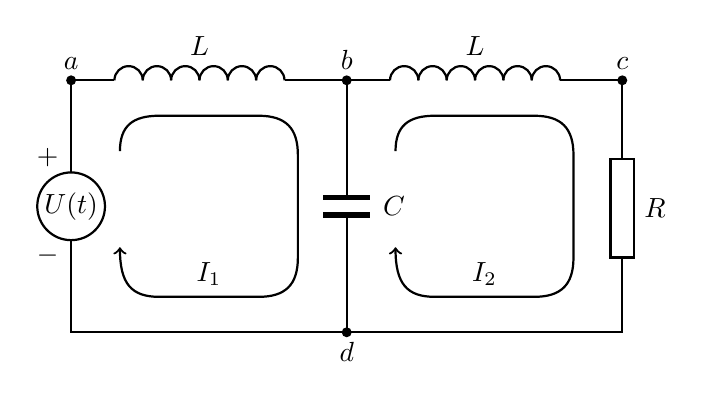
\begin{tikzpicture}[x=1cm,y=1cm,thick]
  % Two series inductors; shunt capacitor bd has a real dielectric gap.
  \draw (0,3.2)--(0.55,3.2);
  \foreach \k in {0,...,5}
    \draw ({0.55+0.36*\k},3.2) arc[start angle=180,end angle=0,radius=0.18];
  \draw (2.71,3.2)--(3.5,3.2)--(4.05,3.2);
  \foreach \k in {0,...,5}
    \draw ({4.05+0.36*\k},3.2) arc[start angle=180,end angle=0,radius=0.18];
  \draw (6.21,3.2)--(7,3.2)--(7,2.2);
  \draw (6.85,0.95) rectangle (7.15,2.2);
  \draw (7,0.95)--(7,0)--(0,0)--(0,1.17);
  \draw (0,1.6) circle (0.43);
  \draw (0,2.03)--(0,3.2);
  \node at (0,1.6) {$U(t)$};
  \node[left] at (-0.03,2.22) {$+$}; \node[left] at (-0.03,0.98) {$-$};
  \draw (3.5,3.2)--(3.5,1.71);
  \draw[line width=2pt] (3.2,1.71)--(3.8,1.71) (3.2,1.49)--(3.8,1.49);
  \draw (3.5,1.49)--(3.5,0);
  \fill (0,3.2) circle (1.8pt) node[above] {$a$};
  \fill (3.5,3.2) circle (1.8pt) node[above] {$b$};
  \fill (7,3.2) circle (1.8pt) node[above] {$c$};
  \fill (3.5,0) circle (1.8pt) node[below] {$d$};
  \node[above] at (1.63,3.38) {$L$}; \node[above] at (5.13,3.38) {$L$};
  \node[right] at (3.83,1.60) {$C$}; \node[right] at (7.15,1.575) {$R$};
  \draw[->] (0.62,2.3)
    .. controls (0.62,2.62) and (0.78,2.75) .. (1.12,2.75)
    --(2.38,2.75)
    .. controls (2.73,2.75) and (2.88,2.59) .. (2.88,2.25)
    --(2.88,0.95)
    .. controls (2.88,0.6) and (2.72,0.45) .. (2.38,0.45)
    --(1.12,0.45)
    .. controls (0.77,0.45) and (0.62,0.61) .. (0.62,1.08);
  \node[above] at (1.75,0.46) {$I_1$};
  \draw[->] (4.12,2.3)
    .. controls (4.12,2.62) and (4.28,2.75) .. (4.62,2.75)
    --(5.88,2.75)
    .. controls (6.23,2.75) and (6.38,2.59) .. (6.38,2.25)
    --(6.38,0.95)
    .. controls (6.38,0.6) and (6.22,0.45) .. (5.88,0.45)
    --(4.62,0.45)
    .. controls (4.27,0.45) and (4.12,0.61) .. (4.12,1.08);
  \node[above] at (5.25,0.46) {$I_2$};
\end{tikzpicture}
